\documentclass[12pt]{article}

\usepackage{booktabs}% http://ctan.org/pkg/booktabs
\usepackage[utf8]{inputenc}
\usepackage{changepage}
\usepackage{pgfplots}
\usepackage{amssymb}
\usepackage{xcolor}
\usepackage{hyperref}
\usepackage{listings}
\usepackage[T1]{fontenc}
\usepackage[utf8]{inputenc}
\usepackage{adjustbox}
\usepackage{amsmath}
\usepackage{mathtools}
\usepackage{biblatex}
\usepackage{float}
\lstset{
  language=Python,
  numbers=left,
  numberstyle=\tiny,
  stepnumber=1,
  numbersep=5pt,
  tabsize=4,
  basicstyle=\ttfamily,
  columns=fullflexible,
  keepspaces,
}
\hypersetup{
    colorlinks,
    citecolor=black,
    filecolor=black,
    linkcolor=black,
    urlcolor=black
}

% Set page size and margins
% Replace `letterpaper' with `a4paper' for UK/EU standard size
\usepackage[letterpaper,top=2cm,bottom=2cm,left=3cm,right=3cm,marginparwidth=1.75cm]{geometry}

% Useful packages
\usepackage{amsmath}
\usepackage{mathtools}
\usepackage{graphicx}
\newenvironment{para}{\begin{adjustwidth}{13mm}{}}{\end{adjustwidth}}

\newcommand\tab[1][1cm]{\hspace*{#1}}

\newcommand{\tabitem}{\llap{\textbullet}}
\newcommand{\Hsquare}{%
\text{\fboxsep=-.2pt\fbox{\rule{0pt}{1ex}\rule{1ex}{0pt}}}%
}

\newtheorem{Definizione}{Definizione}[subsection]
\newtheorem{Lemma}{Lemma}[subsection]
\newtheorem{Teorema/Definizione}{Teorema/Definizione}[subsection]
\newtheorem{Corollario}{Corollario}[subsection]
\newtheorem{Teorema}{Teorema}[subsection]
\newtheorem{Proposizione}{Proposizione}[subsection]
\newtheorem{Notazione}{Notazione}[subsection]
\newtheorem{Commento}{Commento}[subsection]
\newtheorem{Dimostrazione}{Dimostrazione}[subsection]
\newtheorem{Osservazione}{Osservazione}[subsection]
\newtheorem{Nota}{Nota}[subsection]

\title{RSO: Reti}
\author{spitfire}
\date{A.A. 2024-2025}
\begin{document}
\begin{figure}
    \centering
    
\includegraphics[width=0.35\textwidth]{Images/Logo scienze bicocca.png}
\end{figure}

\vspace{10cm}
\date{A.A. 2024-2025}


\maketitle

\newpage

\tableofcontents
\newpage
\section{Introduzione}
Se vogliamo dare una visione "d'insieme" di internet possiamo pensarlo come formato dalle
seguenti componenti:
\begin{itemize}
    \item Miliardi di \textbf{calcolatori} connessi:
    \begin{itemize}
        \item \textbf{Hosts}: dispositivi di computazione e sistemi periferici
        \item Sono sistemi che eseguono \textbf{applicazioni di rete} al "confine" della rete
    \end{itemize}
    \item \textbf{Packet switches}: inoltrano i pacchetti ("pezzi" di dati) tra diversi nodi di rete
    \begin{itemize}
        \item Router, switches, ...
        \item Internet è una \textbf{rete a commutazione di pacchetto}
    \end{itemize}
    \item \textbf{Communication links}: I collegamenti fra i veri nodi della rede
    \begin{itemize}
        \item Fibra, rame, radio, satellite...
        \item \textbf{Transmission rate}: capacità, in termini di bit/s, che il canale può supportare ("larghezza di banda").
    \end{itemize} 
    \item \textbf{Networks}: Collezioni di dispositivi, router, switches e links gestiti \textbf{tutti da una stessa organizzazione}
    \begin{itemize}
        \item Reti residenziali, enterprise ecc... vengono dette solitamente \textbf{reti di accesso}, perché sono quelle reti che raccolgono il traffico
        dagli utenti per mandarlo in rete o viceversa.
    \end{itemize}
\end{itemize}
\begin{center}
    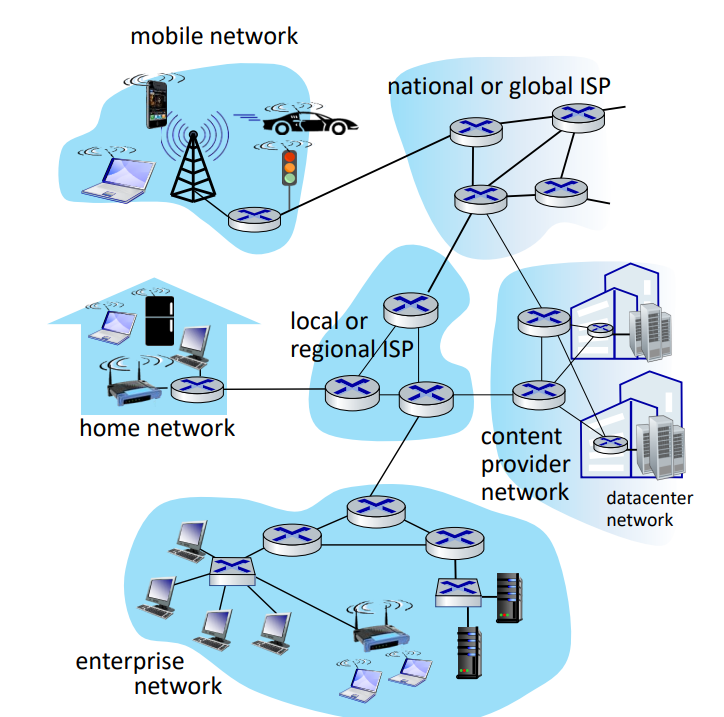
\includegraphics[width = 0.70\linewidth]{Images/1.PNG}
\end{center}
Internet è fisicamente una \textbf{rete connessa}, tuttavia vi sono dei sistemi che permettono di filtrare il traffico (firewall ecc...) per impedire che
ogni nodo della rete sia accessibile da un qualsiasi altro nodo. Internet è quindi una \textbf{rete di reti} che interconnette le reti
degli \textbf{Internet Service Providers} (ISP), cioè quelle entità che forniscono servizi di connettività. Il funzionamento della rete internet è governato
dai \textbf{protocolli di comunicazione}:
\begin{itemize}
    \item Controllano il modo in cui avviene l'invio e il ricevimento dei messaggi
    \item Esempi sono i protocolli HTTP (web), TCP, IP, WiFi, 4G, Ethernet ecc..
\end{itemize}
Protocolli di tipo diverso servono per \textbf{far comunicare dispositivi di tipo diverso}.
Poiché il contesto delle reti è quindi molto eterogeneo, il tutto riesce a funzionare grazie agli \textbf{standard}.
Esistono diversi enti di standardizzazione, tra cui citiamo:
\begin{itemize}
    \item \textbf{RFC}: Request for Comments, documenti
    \item \textbf{IETF}: Internet Engineering Task Force; rilascia le RFC
\end{itemize}
Il compito degli enti di standardizzazione è quello di rilasciare documenti che vanno a definire le caratteristiche
dei protocolli e delle architetture. Possiamo tuttavia vedere internet anche dal punto di vista dei \textbf{servizi}:
internet può essere quindi vista come una \textbf{infrastruttura che offre dei servizi di connettività alle applicazioni distribuite}.
Quindi, internet viene vista come una infrastruttura che \textbf{offre dei servizi di connettività tra nodi diversi}.
\begin{center}
    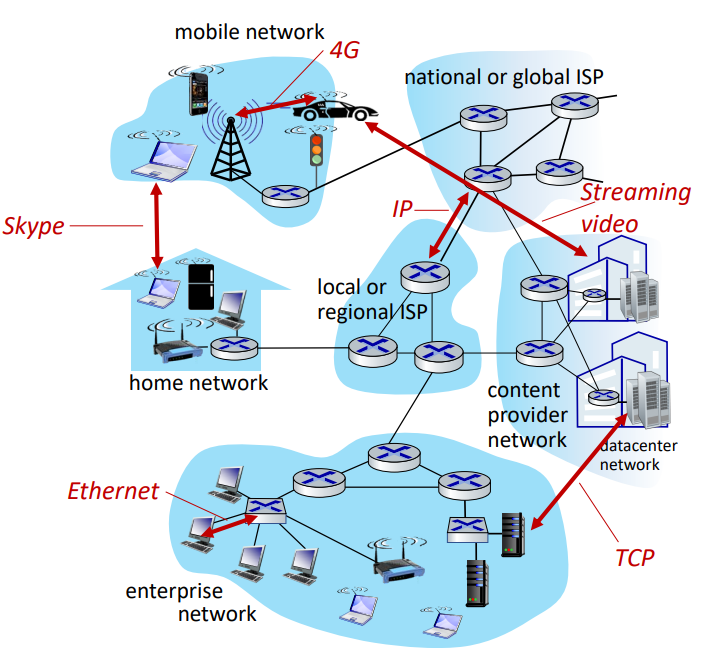
\includegraphics[width = 0.70\linewidth]{Images/2.PNG}
\end{center}
Abbiamo detto che la rete è governata da protocolli, ma \textbf{qual'è la definizione formale di protocollo?}
Una definizione formale può essere la seguente: i \textbf{protocolli} definiscono il \textbf{formato, l'ordine} dei \textbf{messaggi inviati e ricevuti} tra le entità di rete e le
\textbf{azioni intraprese} alla trasmissione e alla ricezione di un messaggio.
\begin{center}
    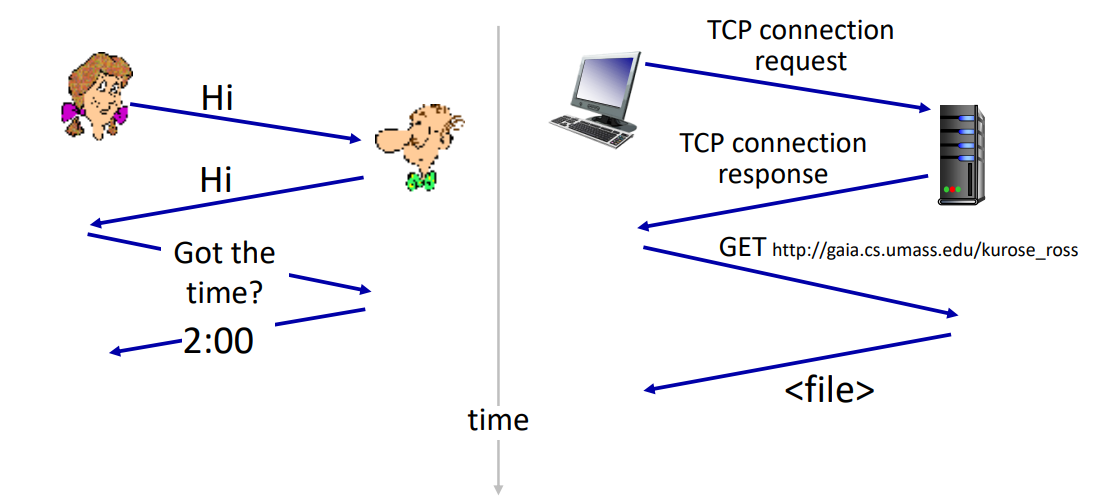
\includegraphics[width = 0.85\linewidth]{Images/3.PNG}
\end{center}
\subsection{Introduzione alla struttura di internet}
La struttura di alto livello di internet si può formalizzare nel seguente modo:
\begin{itemize}
    \item \textbf{Network edge}: il confine della rete, comprende
    \begin{itemize}
        \item \textbf{Hosts}: client e servers
        \item I servers sono spesso in \textbf{data centers}
    \end{itemize}
    È oggetto di dibattito se includere il confine della rete nella struttura di internet o meno; ciò nonostante, rimane comunque
    una componente fondamentale.
    \item \textbf{Access Networks}: Sono tutte quelle reti che servono a raccogliere il traffico generato e destinato per gli utenti.
    Sono quindi i \textbf{punti di accesso alla rete per gli utenti}. Esse possono essere \textbf{cablate oppure wireless}.
    \item \textbf{Network Core}: È l'insieme di tutte quelle reti che sono composte da router interconnessi che permettono di realizzare il concetto di \textbf{rete di reti}.
    Il suo compito è quello di \textbf{connettere le reti di accesso fra di loro} e comprendono tutte quelle reti che, su larga scala, \textbf{permettono il funzionamento di internet}.
\end{itemize}
Ogni componente della struttura di internet viene detto \textbf{segmento}.
\subsubsection{Network Edge}
Il confine della rete è \textbf{popolato dagli host}. Il suo compito principale è quello di inviare i \textbf{pacchetti}
generati dagli host (e quindi dagli utenti). Una visione ad alto livello di questo procedimento è:
\begin{itemize}
    \item Il \textbf{messaggio applicativo} viene generato dall'host
    \item Esso viene \textbf{spezzettato in pezzetti}, chiamati \textbf{pacchetti}, di lunghezza $L$ bits (questa cosa non è sempre vera: ci sono casi in cui i pacchetti hanno lunghezza variabile).
    Ognuno di questi pacchetti presenta una \textbf{intestazione}, cioè un determinato numero di bit che servono per permettere il funzionamento dei protocolli in rete
    \item Una volta generati i pacchetti, essi vengono trasmessi alla rete d'accesso ad un \textbf{tasso di trasmissione} (transmission rate) $R$, il quale è condizionato dalla \textbf{capacità di trasmissione del collegamento}
\end{itemize}
\begin{center}
    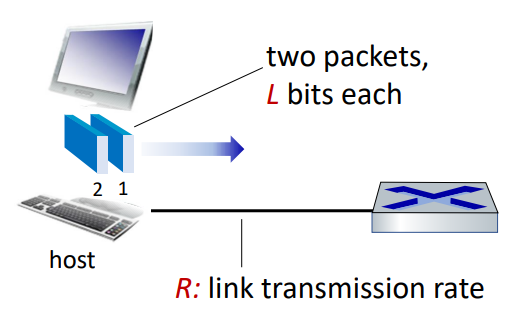
\includegraphics[width = 0.50\linewidth]{Images/4.PNG}
\end{center}
Ogni volta che invio un pacchetto in rete, ho un \textbf{ritardo di trasmissione}, il quale è il tempo necessario per trasmettere un pacchetto di $L$ bit su un collegamento che
ha capacità di trasporto di $R$ bit/sec. Quindi:
$$\textrm{packet transmission delay} = \frac{L \; (bits)}{R \; (bits/sec)}$$
\subsubsection{Access Networks}
Come facciamo a \textbf{connettere gli host a "internet"}? Il compito di effettuare questa connessione è delle
reti di accesso. Esse possono essere:
\begin{itemize}
    \item Reti di accesso \textbf{residenziali}
    \item Reti di accesso \textbf{istituzionali}
    \item Reti di accesso \textbf{mobili}
\end{itemize}
\subsubsection{Network Core}
La Network Core è un insieme di \textbf{maglie di rete interconnesse}, le quali sono fondamentali per effettuare le
operazioni di commutazione dei pacchetti. Esse garantiscono che i pacchetti possano essere trasmessi da un router verso l'altro
attraverso dei collegamenti da una sorgente a una destinazione.
Le reti di core presentano due \textbf{funzionalità fondamentali}:
per spiegarle, dobbiamo prima capire \textbf{come funziona un router}: esso possiede al suo interno una tabella chiamata
\textbf{tabella di inoltro} (forwarding table), che indica verso quale collegamento un pacchetto deve essere instradato in base al valore
della sua intestazione (che quindi contiene, in termini generici, a chi deve essere recapitato questo pacchetto).
L'operazione di \textbf{inoltro} (o \textbf{commutazione di pacchetto}) quindi consiste nell'invio sulla connessione corretta del pacchetto in arrivo (questa operazione viene anche detta \textbf{switching}).
L'inoltro ha \textbf{valenza locale}: ogni router prende in considerazione solo la propria tabella di inoltro locale per decidere dove inoltrare un pacchetto.
Tuttavia, questa operazione non basta per garantire che io possa raggiungere la destinazione corretta; per garantirlo dobbiamo effettuare un'altra operazione che prende il nome di
\textbf{instradamento} (routing). Il routing è un'operazione \textbf{globale} che è utilizzata per determinare \textbf{quale percorso, fra sorgente e destinazione, devono attraversare i pacchetti}.
Ogni singolo router esegui quindi dei \textbf{protocolli} e degli \textbf{algoritmi di routing distribuiti} che hanno l'obbietto di \textbf{popolare le tabelle di inoltro} (viene effettuato tramite algoritmi su grafo).
Poiché gli algoritmi di routing sono \textbf{distribuiti}, essi richiedono lo \textbf{scambio di messaggi e la collaborazione tra i router}.
\begin{center}
    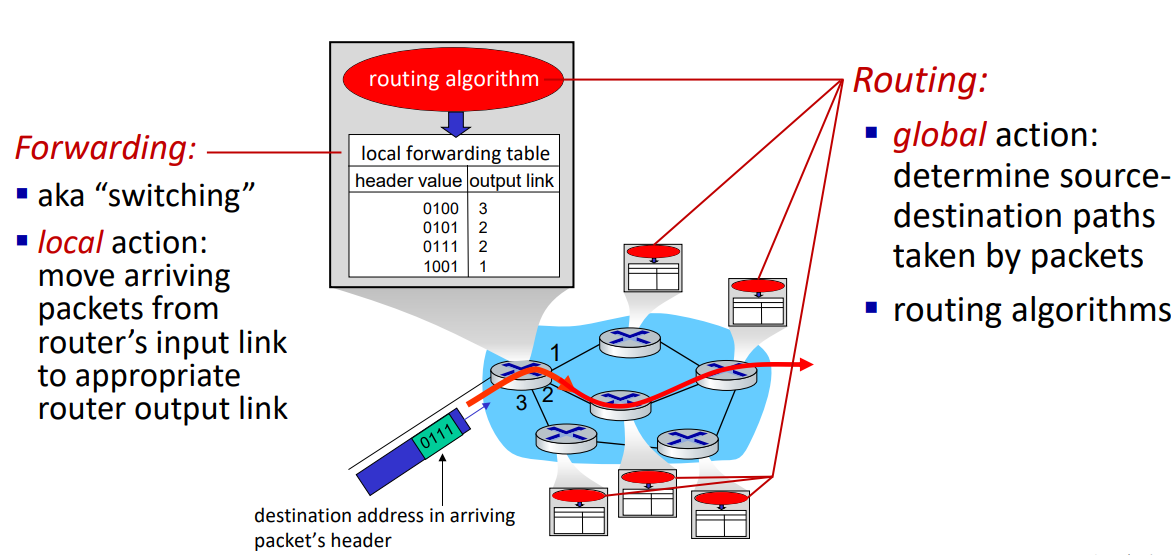
\includegraphics[width = 1\linewidth]{Images/5.PNG}
\end{center}
\subsection{Packet Switching: Store-and-Forward}
Nelle reti a commutazione di pacchetto, \textbf{ogni pacchetto ha vita propria}: una volta che il messaggio viene spezzettato in pacchetti, ognuno di esso
ha un ciclo di vita indipendente dagli altri. La modalità di trasmissione usata da tutte le reti a commutazione di pacchetto è quella del \textbf{store-and-forward}:
quando un pacchetto arriva ad un commutatore per essere commutato, esso deve \textbf{arrivate interamente prima di essere trasmesso al nodo successivo}. Tuttavia, si può pensare
di saltare questo passaggio e trasmettere direttamente ogni bit che arriva su un certo nodo al successivo. Perché non viene fatto nelle reti a commutazione di pacchetto? Il motivo risiede nelle \textbf{intestazioni dei pacchetti}:
infatti, è li che trovo \textbf{tutte le informazioni necessarie per gestire un pacchetto}, quindi devo aspettare che essa venga trasmessa per intero prima di procedere all'invio al nodo successivo.
\begin{center}
    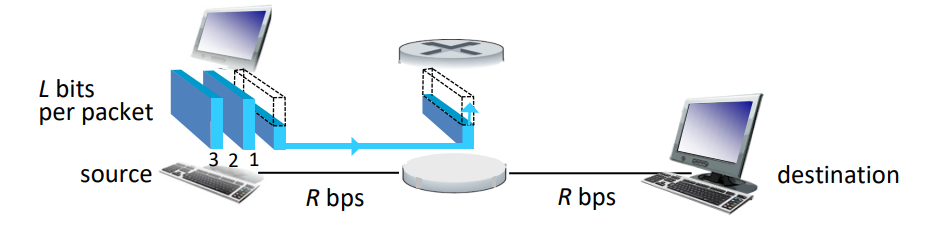
\includegraphics[width =1\linewidth]{Images/6.PNG}
\end{center}
\subsection{Packet-Switching: queuing}
Seppur Store-and-Forward semplifichi di molto la gestione delle reti, esso introduce una problematica che prende il nome di
\textbf{accodamento} (queueing). È una problematica che esiste in tutte le reti e si manifesta quando il \textbf{tasso di arrivo dei pacchetti è superiore al tasso di trasmissione in uscita}.
Nei router e negli switch, i pacchetti si accodano in aree di memoria apposite dette \textbf{buffer}; un pacchetto rimane nel buffer fino a quando non verrà trasmesso.
\begin{center}
    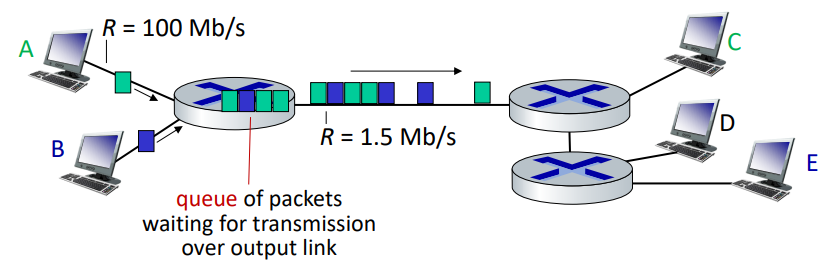
\includegraphics[width =0.90\linewidth]{Images/7.PNG}
\end{center}
Questa è una condizione che può accadere nelle reti a commutazione di pacchetto, tuttavia \textbf{non può essere una situazione sistematica}:
se si verificasse costantemente, la dimensione del buffer \textbf{crescerebbe costantemente} fino a raggiungere la massima dimensione possibile; da quel momento
in poi ogni pacchetto in arrivo porta a una condizione di \textbf{buffer overflow} e andrebbe perso. Quindi, quali sono i problemi che provoca l'accodamento?
\begin{itemize}
    \item \textbf{Buffer overflow} dei buffer dove vengono salvati i pacchetti ancora da trasmettere e susseguente perdita dei pacchetti in arrivo
    \item \textbf{Ritardo di accodamento} dato dall'attesa che il router trasmetta il pacchetto
\end{itemize}
\subsection{Circuit Switching}
La commutazione di pacchetto non è l'unico tipo di commutazione esistente; anzi essa storicamente è posteriore ad un'altro tipo di commutazione
che prende il nome di \textbf{commutazione a circuito}
\begin{center}
    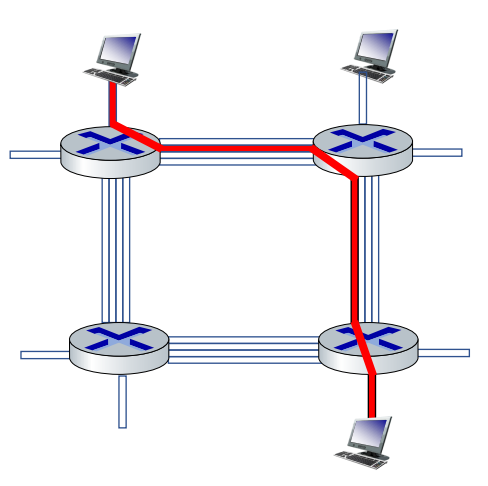
\includegraphics[width =0.45\linewidth]{Images/8.PNG}
\end{center}
Questo tipo di commutazione segue un principio diverso da quella a commutazione di pacchetto: l'elemento fondamentale di questo tipo di rete è il \textbf{circuito} (non esistono i pacchetti in questo tipo di rete).
Tra i vari \textbf{commutatori di circuito} si possono stabilire un certo numero di circuiti.
L'obbiettivo di questo tipo di commutazione è \textbf{destinare i circuiti alla comunicazione tra gli utenti della rete}.
Le risorse di un circuito vengono \textbf{assegnate in maniera esclusiva ad un host} e non possono essere condivise con altri host.
Il vantaggio di questo tipo di commutazione è \textbf{l'assenza di accodamento} data dal completo assegnamento delle risorse di un circuito
ad una sola comunicazione tra sorgente e destinazione.
Viene chiamato \textbf{circuito end-to-end} l'insieme di tutti i circuiti che vengono stabiliti tra sorgente e destinazione.
Uno svantaggio di questo tipo di commutazione è la \textbf{necessità di una fase di setup} in cui vengono allocate le risorse dei circuiti per andare a creare
il circuito end-to-end.
\subsubsection{Packet Switching vs Circuit Switching}
In una commutazione di circuito, le risorse vengono allocate solamente alla comunicazione tra sorgente e destinazione e non esistono
problemi di accodamento. Tuttavia, l'utilizzo delle risorse di rete in questo tipo di comunicazione risulta \textbf{subottimale} rispetto ad una
rete a commutazione di pacchetto. Facciamo un esempio:
\begin{center}
    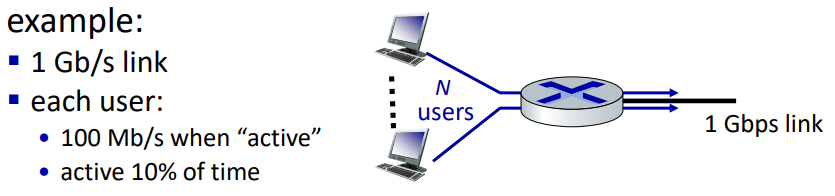
\includegraphics[width =0.75\linewidth]{Images/9.PNG}
\end{center}
\textbf{Domanda: quanti utenti, in queste condizioni, possono rispettivamente accomodare una rete a commutazione di circuito e una rete a commutazione di pacchetto?}
\begin{itemize}
    \item \textbf{Circuit-switching}: 10 utenti
    \item \textbf{Packet-switching}: con 35 utenti, la probabilità che più di 10 utenti siano attivi allo stesso tempo è minore di $0.0004$
\end{itemize}
Quindi una rete a commutazione di pacchetto è sempre la scelta migliore?
\begin{itemize}
    \item Essa è ottima per un traffico di tipo \textbf{"bursty"} (a raffica), cioè in situazioni dove a volte ci sono dati da inviare, a volte no
    \item Permette la condivisione delle risorse di rete
    \item Non richiede setup
\end{itemize}
Tuttavia, se si creano condizioni sfavorevoli, si vanno a creare delle \textbf{situazione di congestione eccessiva della rete}, andando a creare situazioni
di ritardo nella trasmissione dei pacchetti e di buffer overflow. Si rendono quindi necessari \textbf{protocolli di trasmissione affidabili} e meccanismi di \textbf{controllo della congestione}.
È però possibile, visti i vantaggi delle reti a commutazione di circuito, fornire lo stesso tipo di garanzia del servizio anche nelle reti a commutazione di pacchetto?
La risposta è si; esistono delle tecniche che permettono di \textbf{emulare la commutazione di circuito sulle reti a commutazione di pacchetto}, tuttavia sono casi parecchio difficili da gestire.
\subsection{Struttura di internet nel dettaglio}
Gli host sono connessi a internet tramite le \textbf{reti di accesso} fornite da ISPs.
Le reti di accesso devono per forza essere \textbf{interconnesse} per garantire che possa avvenire la comunicazione tra qualsiasi due host della rete (internet è una rete \textbf{connessa}, cioè ogni nodo è raggiungibile da tutti gli altri nodi).
Il risultato dell'evoluzione di internet è una \textbf{struttura gerarchica}; questa evoluzione, tuttavia, non è stata guidata da \textbf{necessità di tipo tecnico} ma di tipo \textbf{economico e politico}.
Vediamo quindi la struttura di internet passo passo: al mondo abbiamo \textbf{milioni} di reti di accesso
\begin{center}
    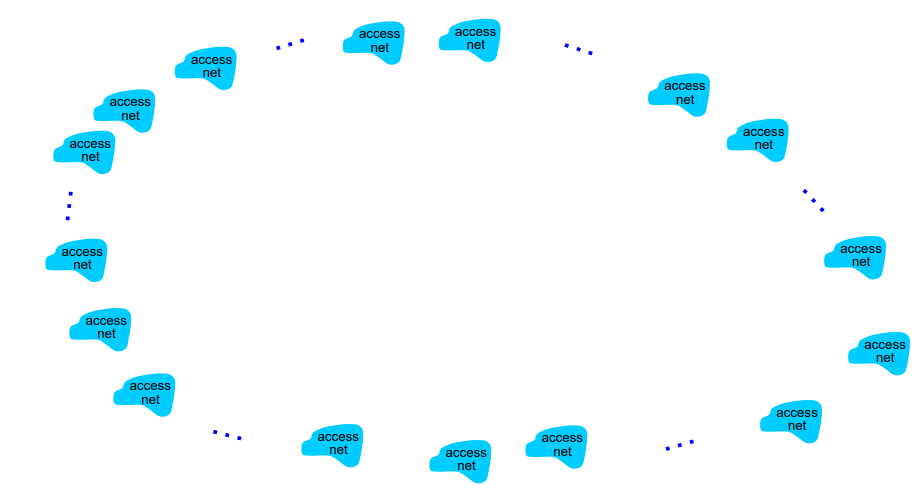
\includegraphics[width =0.85\linewidth]{Images/10.PNG}
\end{center}
L'idea più semplice per interconnetterle è \textbf{connettere ogni ISP agli altri in maniera diretta}, tuttavia...
\begin{center}
    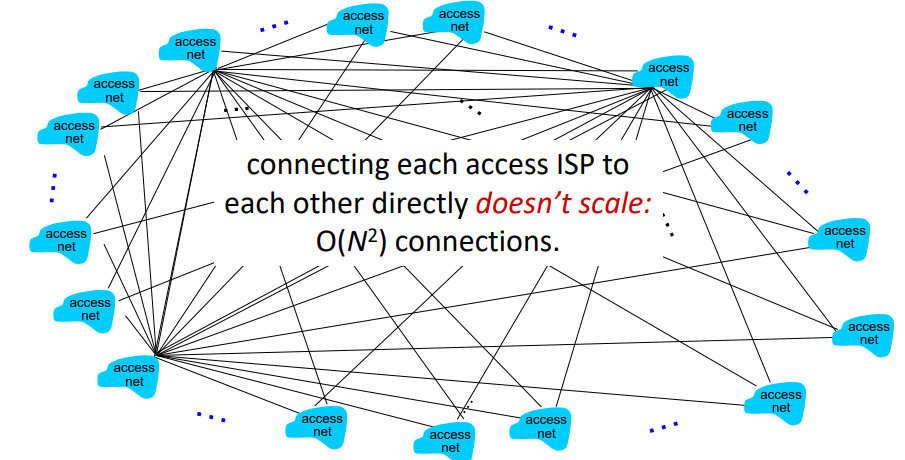
\includegraphics[width =0.85\linewidth]{Images/11.PNG}
\end{center}
Una soluzione alternativa è quella di avere un \textbf{ISP globale} (o di transito) con una rete geograficamente estesa in tutto il mondo, i cui router sono \textbf{interconnessi} e che fornisce connettività alle reti di accesso:
\begin{center}
    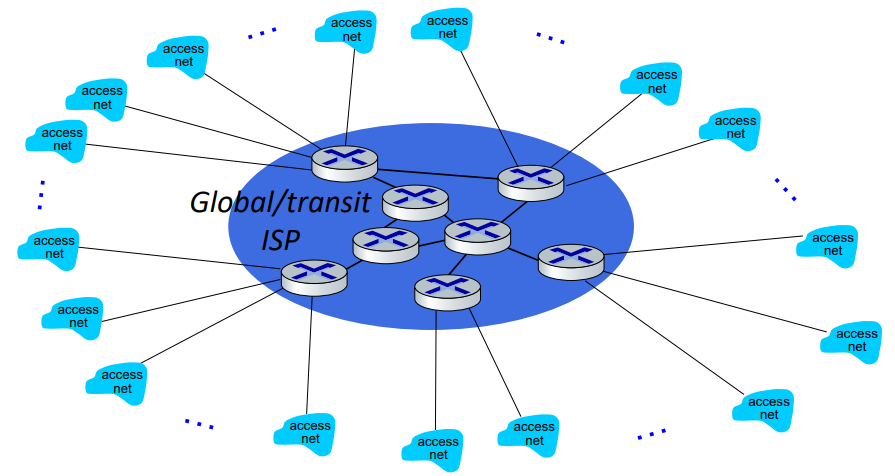
\includegraphics[width =0.85\linewidth]{Images/12.PNG}
\end{center}
Questo approccio tuttavia ha dei problemi:
\begin{itemize}
    \item Richiede una rete estesa \textbf{su tutto il globo}, in modo che possa servire ogni rete di accesso
    \item Richiede un accordo economico tra gli ISP locali e quello globale
    \item Perché ci si dovrebbe limitare ad un solo ISP globale? In effetti, ci potrebbe essere concorrenza fra essi
\end{itemize}
In virtù dell'ultimo punto sopra, si è andata a creare una situazione di questo tipo:
\begin{center}
    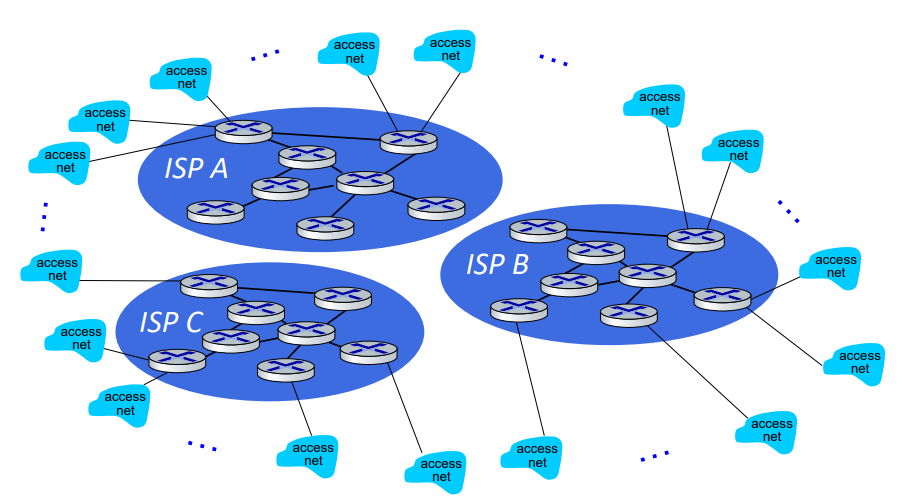
\includegraphics[width =0.85\linewidth]{Images/13.PNG}
\end{center}
si sono andati quindi a creare degli ISPs \textbf{geograficamente estesi} che coprono determinate aree del globo.
Questo genere di ISPs prendono il nome di \textbf{Tier 1 ISPs}.
A questo punto, gli ISPs globali devono creare dei \textbf{peering links} (chiamati così perché \textbf{non sono il frutto di un accordo economico ma di un accordo tra pari})
per creare un'interconnessione tra di loro:
\begin{center}
    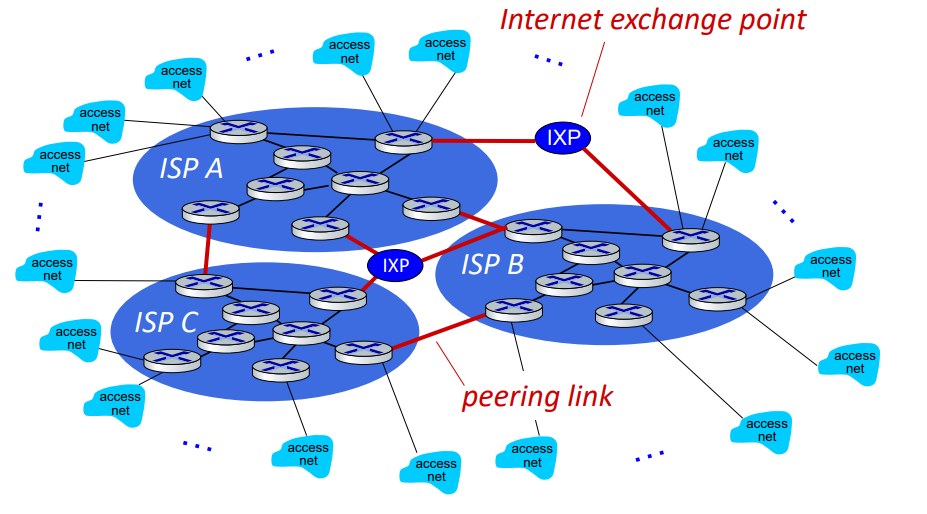
\includegraphics[width =0.85\linewidth]{Images/14.PNG}
\end{center}
Tuttavia, c'è anche un'altra possibilità, cioè quella di avere degli \textbf{Internet Exchange Points} (IXPs), i quali sono dei nodi a cui gli ISPs globali si connettono e che garantiscono
la connessione tra di essi. Tuttavia, tipicamente le reti di acceso non si \textbf{interfacciano direttamente con gli ISPs globali} ma passano tramite \textbf{ISPs regionali}, che hanno una diffusione
più capillare sul territorio. Altro tipo modo in cui le reti di accesso accedono agli ISPs globali è tramite \textbf{multi-homing}, cioè una rete di accesso potrebbe avere \textbf{più collegamenti verso un ISPs globale o regionale};
questo approccio garantisce \textbf{resilienza}
\begin{center}
    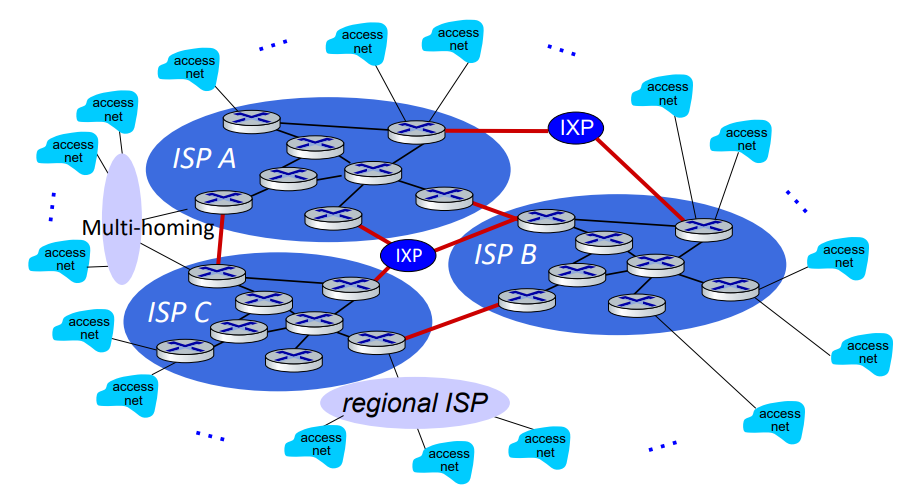
\includegraphics[width =0.85\linewidth]{Images/15.PNG}
\end{center}
Infine, abbiamo le \textbf{reti dei content provider}, che hanno lo scopo di \textbf{fornire contenuto agli utenti}. Per farlo, molto spesso, esse \textbf{bypassano gli ISPs globali} e si interfacciano
direttamente con le reti di accesso.
\begin{center}
    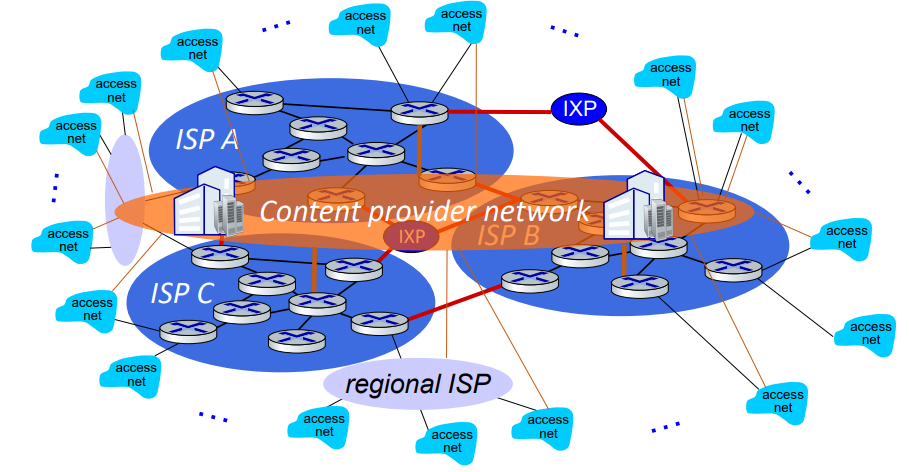
\includegraphics[width =0.85\linewidth]{Images/16.PNG}
\end{center}
Nulla però vieta alle reti dei content provider di accedere anche alle reti degli ISPs globali.
Diamo una versione più generale della gerarchia:
\begin{center}
    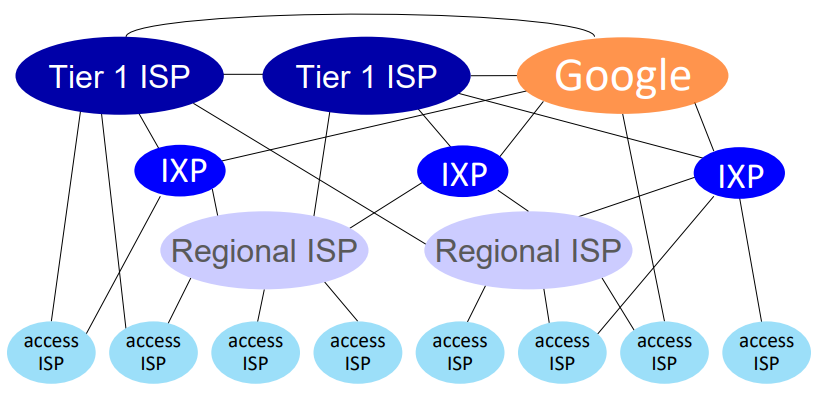
\includegraphics[width =0.85\linewidth]{Images/17.PNG}
\end{center}
Tuttavia, le connessioni possibili \textbf{possono anche non limitarsi a quelle mostrare in figura}.
\end{document}
